\documentclass[11pt]{article}

\usepackage[a4paper,margin=1in]{geometry}
\usepackage[T1]{fontenc}
\usepackage[utf8]{inputenc}
\usepackage{lmodern}
\usepackage{microtype}
\usepackage{amsmath,amssymb,amsthm,mathtools}
\usepackage{booktabs,array}
\usepackage{graphicx}
\usepackage{float}
\usepackage[section]{placeins}
\usepackage{enumitem}
\usepackage[numbers,sort&compress]{natbib}
\usepackage{xcolor}
\usepackage{xurl}
\usepackage[colorlinks=true,linkcolor=blue!55!black,citecolor=blue!55!black,urlcolor=blue!55!black]{hyperref}
\usepackage[nameinlink,noabbrev]{cleveref}

\newtheorem{theorem}{Theorem}[section]
\newtheorem{proposition}[theorem]{Proposition}
\newtheorem{lemma}[theorem]{Lemma}
\newtheorem{corollary}[theorem]{Corollary}
\theoremstyle{definition}
\newtheorem{definition}[theorem]{Definition}
\theoremstyle{remark}
\newtheorem{remark}[theorem]{Remark}

\newcommand{\R}{\mathbb R}
\newcommand{\C}{\mathbb C}
\newcommand{\Id}{\mathrm I}
\newcommand{\cA}{\mathcal A}
\newcommand{\cK}{\mathcal K}
\newcommand{\cG}{\mathcal G}
\newcommand{\cP}{\mathcal P}
\newcommand{\cQ}{\mathcal Q}
\newcommand{\uc}{u_{\mathrm c}}
\newcommand{\norm}[1]{\left\lVert #1\right\rVert}
\newcommand{\spec}{\operatorname{spec}}
\newcommand{\rank}{\operatorname{rank}}
\newcommand{\Ran}{\operatorname{Ran}}
\newcommand{\dist}{\operatorname{dist}}

\title{Validated Isolation of a Negative Continuum Resonance\\
for a Folded-Gaussian Markov Operator\\
\large A Grushin--Rouch\'e Certificate and an Exact Dyadic Galerkin Lift}
\author{Liang Wang}
\date{July 2026}

\begin{document}
\maketitle

\begin{abstract}
A preceding weighted-Riesz analysis reduced the negative peripheral branch
of a folded-Gaussian Markov family to one explicit hypothesis: the full
continuum operator must possess a simple isolated negative resonance, with
enough contour-resolvent control to survive discretization.  Convergent
finite-grid eigenvalues do not prove that statement for a nonnormal
operator.  We close the full-kernel continuum gate at the fixed noise width
$\sigma=10^{-2}$ and at the first band-merging parameter
\[
 \uc^3-2\uc^2+2\uc-2=0.
\]

Let $\cK$ be the exactly normalized folded-Gaussian Markov operator on
$L^\infty([0,1])$ generated by $m(x)=1-\uc x^2$.  For
\[
 c=-0.9865481927458079,\qquad r=0.05,\qquad
 \Gamma=\{z\in\C:|z-c|=r\},
\]
we prove that $\Gamma$ belongs to the resolvent set of $\cK$, that its
interior contains exactly one eigenvalue counted with algebraic
multiplicity, and that
\[
 \sup_{z\in\Gamma}\norm{(z-\cK)^{-1}}_{L^\infty\to L^\infty}
 \le 148.84153451786617.
\]
The operator and the circle are conjugation invariant and the circle lies
strictly in the negative half-plane.  The enclosed eigenvalue is therefore
real, negative, and algebraically simple.

The proof has four independently audited layers.  First, a balanced
rank-one Grushin problem at dimension $4096$ is validated against the exact
stored binary64 Markov matrix.  A componentwise outward residual of
$4.588\times10^{-11}$, a one-center transport product of $0.499527$, and a
scalar Rouch\'e error of $3.278\times10^{-13}$ prove one enclosed matrix
eigenvalue and a contour-resolvent upper of $41.899$.  Second, 224-bit Arb
arithmetic bridges that exact stored matrix to the exact-parameter
continuum-normalized midpoint matrix with row-$\ell^1$ defect at most
$7.315\times10^{-6}$.  Third, cell-average Galerkin matrices satisfy exact
coarse consistency and explicit $L^\infty$ Haar bounds, allowing two Schur
continuations $4096\to8192\to16384$.  Fourth, a finite-rank complement
estimate and a continuum operator defect of $0.012476$ close the final
Neumann gate with product $0.649969$.

This validates the simple-isolated full-kernel parity premise of the
preceding weighted-Riesz theorem.  It also gives a uniform
$L^\infty$ contour theorem for the exact continuum-normalized midpoint
family from dimension $32768$ onward.  The validated norm is not a
dimension-uniform Euclidean norm for the archived sparse matrices.  No
zero-noise limit, zeta-zero identification, self-adjoint
Hilbert--P\'olya operator, or Riemann-hypothesis claim is made.
\end{abstract}

\section{Introduction}
\label{sec:introduction}

The nested-grid program of
\citet{WangNested2026,WangIterated2026} follows a noisy quadratic transfer
operator through dyadic discretizations.  Its physical two-step operator
removes a Perron contribution and a negative peripheral contribution before
squaring the remainder.  A smooth-kernel Haar theorem subsequently
explained the observed quarter--half law
\[
 \norm{E_h},\norm{D_h}=O(h^2),\qquad
 \norm{C_h},\norm{B_h}=O(h),
\]
and a separate Gaussian-tail theorem treated the hard support cutoff
\citep{WangHaar2026,WangCutoff2026}.

The remaining peripheral issue was spectral rather than algebraic.
\citet{WangRiesz2026} replaced gauge-dependent left and right eigenvectors
by the intrinsic weighted Riesz term
\[
 \cQ(A;\Gamma)
 =\frac{1}{2\pi i}\int_\Gamma z(z-A)^{-1}\,dz.
\]
For a smooth compact operator, a simple isolated nonzero eigenvalue gives a
second-order Nystr\"om bridge for this weighted term.  Strong positivity
makes the Perron application unconditional.  The negative branch was left
conditional on a simple isolated continuum resonance.

That condition cannot be inferred from a short table of finite-grid
eigenvalues.  Nonnormal spectra can move much farther than eigenvalue
separation suggests, and a perturbation theorem must see the resolvent
\citep{TrefethenEmbree2005,Kato1995}.  In the present problem the missing
statement has two parts:
\begin{enumerate}[leftmargin=2em]
 \item a contour must contain exactly one eigenvalue of the full continuum
       operator, counted algebraically; and
 \item the resolvent on that contour must have an explicit norm upper that
       survives the finite-to-continuum passage.
\end{enumerate}

We prove both statements by combining a one-center Grushin reduction with a
conditional-expectation Galerkin hierarchy.  The main contributions are:
\begin{enumerate}[leftmargin=2em]
 \item a moment proof of explicit first- and second-derivative row-$L^1$
       bounds for the normalized folded-Gaussian kernel;
 \item exact coarse consistency for cell-average Galerkin operators and
       explicit $L^\infty$ Haar block bounds;
 \item a rank-one Grushin--Rouch\'e theorem that turns one validated inverse
       at the circle center into an exact eigenvalue count and contour
       resolvent;
 \item a 224-bit Arb bridge from the archived sparse binary64 matrix to the
       exact-parameter continuum midpoint matrix;
 \item two dyadic Schur continuations and a final finite-rank-to-continuum
       Neumann transfer; and
 \item a sharp theorem boundary separating the resulting continuum
       $L^\infty$ statement from any unproved dimension-uniform Euclidean
       claim for sparse midpoint matrices.
\end{enumerate}

Three evidence levels are kept separate throughout.
\begin{description}[leftmargin=3.2cm,style=nextline]
 \item[Analytic operator theorem]
 Moment inequalities, Galerkin identities, Schur bounds, perturbation
 invariance, and the continuum conclusion.
 \item[Outward certificate]
 Componentwise binary64 residual enclosures and 224-bit Arb evaluations of
 exact stored and exact-parameter quantities.
 \item[Floating diagnostic]
 The leading-spectrum points used only in the summary figure.  They are
 never used to establish the root count.
\end{description}

\section{The exact operator and the main theorem}
\label{sec:model}

Let
\[
 p(u)=u^3-2u^2+2u-2.
\]
Since
\[
 p'(u)=3u^2-4u+2
      =3\left(u-\frac23\right)^2+\frac23>0,
\]
the polynomial has a unique real root $\uc$ in $(1.5,1.6)$.  Fix
\[
 \sigma=\frac1{100},\qquad m(x)=1-\uc x^2,\qquad 0\le x\le1.
\]
Because $1<\uc<2$, one has
$m([0,1])=[1-\uc,1]\subset[-1,1]$.
For $m\in[-1,1]$, define
\[
 g_m(y)=
 \exp\!\left[-\frac{(y-m)^2}{2\sigma^2}\right]
 +
 \exp\!\left[-\frac{(y+m)^2}{2\sigma^2}\right],
 \qquad 0\le y\le1,
\]
\[
 Z(m)=\int_0^1g_m(y)\,dy,
 \qquad
 k(x,y)=\frac{g_{m(x)}(y)}{Z(m(x))}.
\]
The continuum Markov operator is
\begin{equation}
 (\cK f)(x)=\int_0^1k(x,y)f(y)\,dy
 \quad\text{on }L^\infty([0,1]).
 \label{eq:continuum-operator}
\end{equation}
Its kernel is real, strictly positive, and smooth on the compact square.
Thus $\cK$ is a compact Markov operator; in particular,
$\norm{\cK}_{\infty\to\infty}=1$.

The numerical contour data are
\begin{equation}
 c=-0.9865481927458079,\qquad
 r=0.05,\qquad
 \Gamma=\{z\in\C:|z-c|=r\}.
 \label{eq:main-contour}
\end{equation}
The certificate treats the round-trip binary64 values represented by the
displayed decimals as exact real inputs and rounds every subsequent
inequality outward.  The contour obeys
\[
 \min_{z\in\Gamma}|z|
 \ge0.9365481927458077,
 \qquad
 \max_{z\in\Gamma}\operatorname{Re}z
 =-0.9365481927458078<0.
\]

\begin{theorem}[Validated negative continuum resonance]
\label{thm:main}
For the exact operator \eqref{eq:continuum-operator} at
$\sigma=1/100$ and the exact critical parameter $\uc$:
\begin{enumerate}[label=\textup{(\roman*)}]
 \item $\Gamma\subset\rho(\cK)$;
 \item the Riesz projection
 \[
   \Pi_\Gamma(\cK)
   =\frac{1}{2\pi i}\int_\Gamma(z-\cK)^{-1}\,dz
 \]
 has rank one;
 \item the interior of $\Gamma$ contains one real negative algebraically
 simple eigenvalue $\lambda_-$; and
 \item
 \[
  \sup_{z\in\Gamma}\norm{(z-\cK)^{-1}}_{\infty\to\infty}
  \le148.84153451786617.
 \]
\end{enumerate}
\end{theorem}

The proof is completed in \cref{sec:continuum-closure}.  The reality
conclusion does not require a separate numerical enclosure of the imaginary
part: a real operator has conjugate-paired spectrum, while a
conjugation-invariant disk of algebraic count one cannot contain a nonreal
pair.

\begin{corollary}[Closure of the full-kernel parity premise]
\label{cor:riesz}
At $\sigma=1/100$, the simple-isolated negative-resonance premise in the
full-kernel parity corollary of \citet{WangRiesz2026} is satisfied.  Hence
the gauge-free weighted Nystr\"om term for this branch has the
second-order full-kernel continuum bridge proved there.
\end{corollary}

\begin{remark}[Norm boundary]
\label{rem:norm-boundary}
\Cref{thm:main} is an $L^\infty$ operator theorem.  It does not assert a
dimension-uniform $\ell^2$ resolvent bound for the support-truncated stored
matrices.  This distinction is essential for a nonnormal family.
\end{remark}

\section{Moment and derivative bounds for the folded kernel}
\label{sec:derivatives}

The continuum step requires explicit row-integrated derivative bounds rather
than pointwise Gaussian peaks.  They follow from a truncated-normal moment
inequality.

Let $T$ have density
\[
 \pi_m(t)=\frac{\exp[-(t-m)^2/(2\sigma^2)]}
 {\int_{-1}^1\exp[-(s-m)^2/(2\sigma^2)]\,ds},
 \qquad -1\le t\le1,
\]
where $m\in[-1,1]$.  Folding $T$ by $t\mapsto|t|$ gives the density
$g_m/Z(m)$ on $[0,1]$.

\begin{lemma}[Truncated second moment]
\label{lem:moment}
For every $m\in[-1,1]$,
\[
 \mathbb E(T-m)^2\le\sigma^2,
 \qquad
 \operatorname{Var}(T)\le\sigma^2.
\]
\end{lemma}

\begin{proof}
Put $X=(T-m)/\sigma$.  Its conditioning interval is $[a,b]$ with
$a\le0\le b$.  Since
\[
 \int_a^b(x^2-1)e^{-x^2/2}\,dx
 =[-xe^{-x^2/2}]_a^b
 =-be^{-b^2/2}+ae^{-a^2/2}\le0,
\]
the conditional expectation satisfies $\mathbb E X^2\le1$.  This proves the
first inequality, and variance is no larger than the second moment about
$m$.
\end{proof}

\begin{lemma}[Normalized folded derivative envelope]
\label{lem:folded-derivatives}
Write $q_m(y)=g_m(y)/Z(m)$.  Then
\begin{align}
 \norm{\partial_m q_m}_{L^1(0,1)},
 \ \norm{\partial_y q_m}_{L^1(0,1)}
 &\le \sigma^{-1},
 \label{eq:first-folded}\\
 \norm{\partial_{mm}q_m}_{L^1(0,1)},
 \ \norm{\partial_{my}q_m}_{L^1(0,1)},
 \ \norm{\partial_{yy}q_m}_{L^1(0,1)}
 &\le2\sigma^{-2}.
 \label{eq:second-folded}
\end{align}
\end{lemma}

\begin{proof}
Let $\mu=\mathbb ET$ and $v=\operatorname{Var}(T)$.  Before folding, the
parameter score identities are
\[
 \partial_m\pi_m(t)=\frac{t-\mu}{\sigma^2}\pi_m(t),
\]
\[
 \partial_{mm}\pi_m(t)
 =\frac{(t-\mu)^2-v}{\sigma^4}\pi_m(t).
\]
By \cref{lem:moment}, Cauchy--Schwarz gives the first parameter bound and
\[
 \norm{\partial_{mm}\pi_m}_1
 \le\frac{2v}{\sigma^4}\le\frac2{\sigma^2}.
\]
The target identities are
\[
 \partial_t\pi_m(t)
 =-\frac{t-m}{\sigma^2}\pi_m(t),
\qquad
 \partial_{tt}\pi_m(t)
 =\left(\frac{(t-m)^2}{\sigma^4}-\frac1{\sigma^2}\right)\pi_m(t),
\]
and
\[
 \partial_{mt}\pi_m(t)
 =\left(
 \frac1{\sigma^2}
 -\frac{(t-m)(t-\mu)}{\sigma^4}
 \right)\pi_m(t).
\]
Again \cref{lem:moment} and Cauchy--Schwarz give the displayed bounds.
Pushforward by the folding map cannot increase total variation, so the same
$L^1$ inequalities hold for $q_m$.
\end{proof}

For $m(x)=1-\uc x^2$, use the validated analytic upper
$\uc<1.544$.  Define
\[
 L_x=\sup_x\int_0^1|\partial_xk(x,y)|\,dy,
 \quad
 L_y=\sup_x\int_0^1|\partial_yk(x,y)|\,dy,
\]
and analogously $L_{xx},L_{xy},L_{yy}$.

\begin{corollary}[Numerical derivative ledger]
\label{cor:derivative-ledger}
The exact continuum kernel satisfies the outward bounds
\begin{align*}
 L_x&\le308.80000000000024,
 &L_y&\le100.00000000000001,\\
 L_{xx}&\le191023.68000000023,
 &L_{xy}&\le61760.000000000044,\\
 L_{yy}&\le20000.000000000004.
\end{align*}
\end{corollary}

\begin{proof}
The chain rule and \cref{lem:folded-derivatives} give
\[
 L_x\le2u\sigma^{-1},\qquad
 L_{xx}\le4u^2(2\sigma^{-2})+2u\sigma^{-1},
\]
\[
 L_{xy}\le2u(2\sigma^{-2}),\qquad
 L_y\le\sigma^{-1},\qquad
 L_{yy}\le2\sigma^{-2}.
\]
Insert $u=1.544$ and $\sigma=1/100$, rounding upward.
\end{proof}

\section{Cell-average Galerkin and contour transport}
\label{sec:galerkin}

Let $I_i=[ih,(i+1)h)$, $h=1/n$, and let $P_n$ be conditional expectation
onto functions constant on the cells $I_i$.  The finite-rank operator
\[
 \cA_n=P_n\cK P_n
\]
is represented on cell values by the row-stochastic matrix
\begin{equation}
 (A_n)_{ij}
 =\frac1h\int_{I_i}\int_{I_j}k(x,y)\,dy\,dx.
 \label{eq:galerkin-matrix}
\end{equation}
The continuum-normalized midpoint matrix is
\begin{equation}
 (M_n)_{ij}=h\,k(x_i,y_j),
 \qquad
 x_i=y_i=\left(i+\frac12\right)h.
 \label{eq:midpoint-matrix}
\end{equation}
All matrix norms in this paper are induced row-$\ell^\infty$ norms unless
another norm is explicitly written.

\begin{proposition}[Midpoint and continuum defects]
\label{prop:defects}
The derivative constants of \cref{cor:derivative-ledger} give
\begin{align}
 \norm{M_n-A_n}_\infty
 &\le\frac{h^2}{8}(L_{xx}+L_{yy}),
 \label{eq:midpoint-galerkin}\\
 \norm{\cK-P_n\cK P_n}_{\infty\to\infty}
 &\le\frac h2(L_x+L_y).
 \label{eq:continuum-galerkin}
\end{align}
\end{proposition}

\begin{proof}
For \eqref{eq:midpoint-galerkin}, apply the one-dimensional midpoint
remainder successively in $x$ and $y$ on every cell rectangle.  The
entrywise error is bounded by
$h^3(L_{xx}+L_{yy})/8$; summing one matrix row over $n=1/h$ cells gives the
claim.

For \eqref{eq:continuum-galerkin}, write
\[
 \cK-P_n\cK P_n=(\Id-P_n)\cK+P_n\cK(\Id-P_n).
\]
Output averaging costs at most $hL_x/2$.  On each input cell,
$f-P_nf$ has mean zero, so subtracting a cellwise constant from
$k(x,\cdot)$ and using the target derivative costs at most $hL_y/2$.
\end{proof}

The advantage of cell averages over midpoint samples is exact nesting.
Let $J,W:\C^n\to\C^{2n}$ be replication and alternating-detail injections,
\[
 (Jv)_{2i}=(Jv)_{2i+1}=v_i,\qquad
 (Wv)_{2i}=v_i,\quad(Wv)_{2i+1}=-v_i,
\]
with restrictions $R=J^*/2$ and $S=W^*/2$.  In these coordinates,
\begin{equation}
 \begin{bmatrix}R\\S\end{bmatrix}
 A_{2n}[J\ W]
 =
 \begin{pmatrix}
 A_n&B_n\\
 C_n&D_n
 \end{pmatrix}.
 \label{eq:haar-blocks}
\end{equation}
The upper-left identity is exact because
$P_nP_{2n}=P_n$.

\begin{proposition}[Exact-consistency Haar bounds]
\label{prop:haar}
For a coarse mesh $h=1/n$,
\begin{equation}
 \norm{C_n}_\infty\le\frac h4L_x,\qquad
 \norm{B_n}_\infty\le\frac h2L_y,\qquad
 \norm{D_n}_\infty\le\frac{h^2}{8}L_{xy}.
 \label{eq:haar-bounds}
\end{equation}
The coarse-consistency defect in \eqref{eq:haar-blocks} is exactly zero.
\end{proposition}

\begin{proof}
The $C_n$ block contains one signed difference between the two source
half-cells, the $B_n$ block one mean-zero target-cell cancellation, and the
$D_n$ block both cancellations.  Integrating the corresponding first or
mixed derivative over the half-cell rectangles gives
\eqref{eq:haar-bounds}.  Exact coarse consistency follows from the tower
property of conditional expectation.
\end{proof}

We use two standard contour-transfer lemmas.  They are stated explicitly to
keep every nonnormal constant visible.

\begin{lemma}[Neumann contour transfer]
\label{lem:neumann}
Let $\Gamma\subset\rho(A)$ and
\[
 M=\sup_{z\in\Gamma}\norm{(z-A)^{-1}}.
\]
If $\norm{B-A}\le\delta$ and $M\delta<1$, then
$\Gamma\subset\rho(B)$,
\[
 \sup_{z\in\Gamma}\norm{(z-B)^{-1}}
 \le\frac{M}{1-M\delta},
 \label{eq:neumann-resolvent}
\]
and the Riesz projections of $A$ and $B$ inside $\Gamma$ have the same
finite rank.
\end{lemma}

\begin{proof}
Factor $z-B=(z-A)[\Id-(z-A)^{-1}(B-A)]$ and use a Neumann series uniformly
on the contour.  The same estimate applies to the homotopy
$A+t(B-A)$, $0\le t\le1$, so the Riesz rank is constant
\citep{Kato1995}.
\end{proof}

\begin{lemma}[One dyadic Schur step]
\label{lem:schur}
Suppose the coarse contour resolvent is bounded by $M$, and put
\[
 \rho=\min_{z\in\Gamma}|z|,\quad
 b=\norm{B_n}_\infty,\quad
 c_1=\norm{C_n}_\infty,\quad
 d=\norm{D_n}_\infty.
\]
If $d<\rho$, set
\[
 R_d=\frac1{\rho-d},\qquad
 \varepsilon=bR_dc_1.
\]
If $M\varepsilon<1$, the fine and coarse matrices have the same count inside
$\Gamma$.  Moreover, with
\[
 S=\frac{M}{1-M\varepsilon},
\]
the fine resolvent is bounded by
\begin{equation}
 S+SbR_d+R_dc_1S+
 R_d+R_dc_1SbR_d.
 \label{eq:schur-resolvent}
\end{equation}
\end{lemma}

\begin{proof}
Take the Schur complement of $z-D_n$.  Its inverse is bounded by $R_d$,
and its self-energy has norm at most $\varepsilon$.  Apply
\cref{lem:neumann} to the coarse Schur complement and then bound the four
blocks of the inverse.  For count preservation, use the homotopy
\[
 \begin{pmatrix}A_n&tB_n\\tC_n&tD_n\end{pmatrix},
 \qquad0\le t\le1.
\]
Every displayed bound is dominated by its value at $t=1$, so the contour
remains in the resolvent set throughout.  Formula
\eqref{eq:schur-resolvent} also includes the exact conversion from
coarse/detail coordinates back to the fine $\ell^\infty$ coordinates.
\end{proof}

\begin{lemma}[The zero complement]
\label{lem:zero-complement}
If the Galerkin matrix $A_n$ has contour-resolvent upper $M_n$, then the
finite-rank operator $\cA_n=P_n\cK P_n$ on all of $L^\infty$ satisfies
\begin{equation}
 \sup_{z\in\Gamma}\norm{(z-\cA_n)^{-1}}_{\infty\to\infty}
 \le M_n+\frac2{\rho},
 \qquad
 \rho=\min_{z\in\Gamma}|z|.
 \label{eq:zero-complement}
\end{equation}
\end{lemma}

\begin{proof}
On $\Ran P_n$, the operator is represented by $A_n$; on $\ker P_n$ it is
zero.  Therefore
\[
 (z-\cA_n)^{-1}
 =J_n(z-A_n)^{-1}P_n+z^{-1}(\Id-P_n),
\]
where $J_n$ includes cell values as piecewise-constant functions.  Since
$\norm{P_n}=1$ and $\norm{\Id-P_n}\le2$, \eqref{eq:zero-complement}
follows.
\end{proof}

\section{The exact stored Grushin certificate}
\label{sec:grushin}

Let $P^{\mathrm s}_{4096}$ denote the sparse Markov matrix archived in the
RH-36 snapshot.  In this section every stored binary64 entry is treated as
an exact real number.  The second stored peripheral mode supplies a center
$c$, right vector $r_0$, and left vector $\ell_0$.  No assumption that these
are exact eigenvectors is made.

With the exactly representable scale $s=16$, define the bordered problem
\begin{equation}
 \cG(z)=
 \begin{pmatrix}
 z\Id-P^{\mathrm s}_{4096}&s r_0\\
 s^{-1}\ell_0^T&0
 \end{pmatrix}.
 \label{eq:grushin}
\end{equation}
Write its inverse blocks as
\[
 \cG(z)^{-1}
 =
 \begin{pmatrix}
 E(z)&E_+(z)\\
 E_-(z)&E_{-+}(z)
 \end{pmatrix}.
\]

\begin{proposition}[One-center Grushin--Rouch\'e criterion]
\label{prop:grushin}
Let
\[
 g_- \le \ell_0^Tr_0\le g_+,\qquad
 \delta_r=\norm{(P^{\mathrm s}_{4096}-c\Id)r_0}_\infty,
\]
\[
 \delta_\ell=
 \norm{((P^{\mathrm s}_{4096})^T-c\Id)\ell_0}_1,
\qquad
 e_0\ge\norm{E(c)}_\infty.
\]
If $re_0<1$, put
\[
 M_E=\frac{e_0}{1-re_0},
\]
\[
 M_+=\frac{s\norm{r_0}_\infty}{g_-}
      +\frac{M_Es\delta_r}{g_-},
\qquad
 M_-=\frac{\norm{\ell_0}_1}{sg_-}
      +\frac{\delta_\ell M_E}{sg_-},
\]
\[
 \varepsilon_*=\frac{M_-s\delta_r}{g_-}.
\]
If
\[
 \varepsilon_*<\frac r{g_+},
 \label{eq:rouche-gate}
\]
then the disk $|z-c|<r$ contains exactly one eigenvalue of
$P^{\mathrm s}_{4096}$ counted algebraically, and
\begin{equation}
 \sup_{|z-c|=r}\norm{(z-P^{\mathrm s}_{4096})^{-1}}_\infty
 \le
 M_E+\frac{M_+M_-}{r/g_+-\varepsilon_*}.
 \label{eq:grushin-resolvent}
\end{equation}
\end{proposition}

\begin{proof}
The bordered resolvent identity gives
\[
 E(z)=E(c)[\Id+(z-c)E(c)]^{-1}.
\]
Thus $re_0<1$ keeps $\cG(z)$ invertible on the closed disk and bounds the
leading block by $M_E$.  Applying the exact bordered inverse identities to
$r_0$ and $\ell_0$ gives the channel bounds $M_+$ and $M_-$.  Applying
$\cG(z)^{-1}$ to the candidate border column
\[
 \begin{pmatrix}
 sr_0/g\\-(z-c)/g
 \end{pmatrix},
 \qquad g=\ell_0^Tr_0,
\]
shows that on the boundary
\[
 \left|E_{-+}(z)+\frac{z-c}{g}\right|
 \le\varepsilon_*.
\]
Condition \eqref{eq:rouche-gate} and scalar Rouch\'e imply that
$E_{-+}$ has one zero in the disk \citep{Ahlfors1979}.  Since the bordered
problem has no pole there, zeros of the effective scalar are eigenvalues of
the original matrix with algebraic multiplicity
\citep{SjoestrandZworski2007,GohbergSigal1971}.  Finally,
\[
 (z-P^{\mathrm s}_{4096})^{-1}
 =E(z)-E_+(z)E_{-+}(z)^{-1}E_-(z),
\]
which gives \eqref{eq:grushin-resolvent}.
\end{proof}

The approximate inverse of $\cG(c)$ is generated by sparse LU.  Its
residual is then recomputed against the exact stored graph
\[
 cX-P^{\mathrm s}_{4096}X+s r_0\alpha,
 \qquad
 s^{-1}\ell_0^TX,
\]
using componentwise outward arithmetic
\citep{Rump2010,WangOutward2026}.  In particular, the rounded sparse assembly used
to generate the LU factor is not reused as the exact target.

\begin{table}[H]
\centering
\caption{Exact-stored $4096$ Grushin ledger.  All displayed inequalities are
outward upper or lower bounds.}
\label{tab:grushin}
\begin{tabular}{@{}lr@{}}
\toprule
quantity & certified value\\
\midrule
bordered inverse residual $\norm{\Id-\cG(c)X}_\infty$
  & $4.587902979431811\times10^{-11}$\\
$\norm{\cG(c)^{-1}}_\infty$
  & $\le10.263377331567700$\\
center reduced inverse $e_0$
  & $\le9.990523884439735$\\
center transport product $re_0$
  & $\le0.499526194221987$\\
right mode residual $\delta_r$
  & $\le5.098820251133382\times10^{-15}$\\
left mode residual $\delta_\ell$
  & $\le3.817629187162489\times10^{-11}$\\
Gram interval $\ell_0^Tr_0$
  & $[1.000000000000002,\ 1.0000000000000024]$\\
effective-scalar error $\varepsilon_*$
  & $\le3.277264606378967\times10^{-13}$\\
effective-scalar boundary lower
  & $\ge0.04999999999967214$\\
stored contour resolvent
  & $\le41.89853481734383$\\
\bottomrule
\end{tabular}
\end{table}

\begin{corollary}[Stored count]
\label{cor:stored}
The exact stored binary64 matrix $P^{\mathrm s}_{4096}$ has exactly one
eigenvalue in the disk \eqref{eq:main-contour}, counted algebraically, and
its contour resolvent is bounded by $41.89853481734383$.
\end{corollary}

\section{Arb bridge to the exact-parameter midpoint matrix}
\label{sec:arb-bridge}

The stored matrix uses a binary64 approximation of $\uc$, a support window,
binary64 Gaussian values, and discrete row normalization.  To connect
\cref{cor:stored} to the analytic operator, all of these effects are enclosed
in one row-$\ell^1$ comparison with the exact matrix
\eqref{eq:midpoint-matrix}.

At 224-bit precision, Arb \citep{Johansson2017} validates
\begin{align*}
 1.543689012692076361570855971801747986525203297650983935240803
 <\uc\\
 {}<
 1.543689012692076361570855971801747986525203297650983935240805.
\end{align*}
The polynomial balls at the endpoints are respectively
\[
 [-3.08669\times10^{-60}\ \mathord{+/-}\ 3.14\times10^{-66}]
\]
and
\[
 [2.861655\times10^{-60}\ \mathord{+/-}\ 6.08\times10^{-67}].
\]
Together with $p'>0$, this proves the exact root bracket.

The archived support has half-width $330$ midpoint cells.  Arb verifies its
contiguous support geometry in every one of the $4096$ rows throughout the
root interval.  The smallest distance of a folded center from an ambiguous
floor boundary is
\[
 9.718324434970780\times10^{-6}.
\]
A Gaussian sum--integral tail estimate gives the uniform omitted exact
midpoint mass
\[
 \tau_{\mathrm{omit}}
 \le1.9049777585621693\times10^{-15}.
\]
Every retained stored binary64 entry is then subtracted from the exact Arb
ball
\[
 h\frac{
 e^{-(y_j-m(x_i))^2/(2\sigma^2)}
 +e^{-(-y_j-m(x_i))^2/(2\sigma^2)}
 }{Z(m(x_i))}
\]
and the absolute balls are summed rowwise.

\begin{proposition}[Exact stored-to-midpoint bridge]
\label{prop:stored-midpoint}
For the exact stored binary64 matrix and the exact-parameter
continuum-normalized midpoint matrix,
\begin{equation}
 \norm{P^{\mathrm s}_{4096}-M_{4096}}_\infty
 \le7.314948554132701\times10^{-6}.
 \label{eq:stored-midpoint}
\end{equation}
The largest enclosed row is row $302$.
\end{proposition}

This is an Arb statement about exact stored numbers and exact analytic
parameters.  It is not a floating residual estimate.

Combining \cref{eq:stored-midpoint} with
\cref{eq:midpoint-galerkin} gives
\[
 \norm{P^{\mathrm s}_{4096}-A_{4096}}_\infty
 \le
 7.314948554132701\times10^{-6}
 +0.0015722489356994657
\]
\begin{equation}
 \hspace{3cm}
 =0.0015795638842535985.
 \label{eq:stored-galerkin-total}
\end{equation}
The product with the stored contour-resolvent upper is
\[
 41.89853481734383
 \times0.0015795638842535985
 \le0.06618141240061828<1.
\]
Therefore \cref{lem:neumann} proves:

\begin{corollary}[Galerkin count at $4096$]
\label{cor:galerkin4096}
The cell-average Galerkin matrix $A_{4096}$ has one eigenvalue inside
$\Gamma$, counted algebraically, and
\[
 \sup_{z\in\Gamma}\norm{(z-A_{4096})^{-1}}_\infty
 \le44.86795976620544.
\]
\end{corollary}

\section{Dyadic continuation and continuum closure}
\label{sec:continuum-closure}

The exact-consistency hierarchy now propagates
\cref{cor:galerkin4096} without constructing matrices at dimensions $8192$
or $16384$.  \Cref{tab:schur} lists the analytic block and Schur bounds.

\begin{table}[H]
\centering
\caption{Two exact-consistency dyadic Schur steps.  Here $C$ maps coarse
input to detail output and $B$ maps detail input to coarse output.}
\label{tab:schur}
\scriptsize
\setlength{\tabcolsep}{3.5pt}
\begin{tabular}{@{}lrrrrrr@{}}
\toprule
step & $\norm C_\infty$ & $\norm B_\infty$ & $\norm D_\infty$
& self-energy & product & fine resolvent\\
\midrule
$4096\to8192$
& $1.88477{\times}10^{-2}$
& $1.22070{\times}10^{-2}$
& $4.60148{\times}10^{-4}$
& $2.45782{\times}10^{-4}$
& $0.0110278$
& $47.95355$\\
$8192\to16384$
& $9.42383{\times}10^{-3}$
& $6.10352{\times}10^{-3}$
& $1.15037{\times}10^{-4}$
& $6.14229{\times}10^{-5}$
& $0.00294545$
& $49.96374$\\
\bottomrule
\end{tabular}
\end{table}

Both Schur products are below one.  Hence the algebraic count remains one
at both levels.  The resulting $16384$ Galerkin matrix resolvent satisfies
\begin{equation}
 M_{16384}\le49.963731139831324.
 \label{eq:galerkin16384}
\end{equation}

The matrix estimate must still be lifted to the operator on all of
$L^\infty$.  The minimum contour modulus is
\[
 \rho\ge0.9365481927458077.
\]
By \cref{lem:zero-complement}, the zero action on $\ker P_{16384}$ adds
\[
 \frac2\rho\le2.135501424797291,
\]
so
\begin{equation}
 \sup_{z\in\Gamma}
 \norm{(z-P_{16384}\cK P_{16384})^{-1}}_{\infty\to\infty}
 \le52.09923256462863.
 \label{eq:finite-rank-resolvent}
\end{equation}
The analytic continuum defect is
\begin{equation}
 \norm{\cK-P_{16384}\cK P_{16384}}_{\infty\to\infty}
 \le0.012475585937500016.
 \label{eq:final-defect}
\end{equation}
The final Neumann product is therefore
\begin{equation}
 52.09923256462863
 \times0.012475585937500016
 \le0.649968453137824<1.
 \label{eq:final-product}
\end{equation}
Applying \cref{lem:neumann} gives
\[
 \sup_{z\in\Gamma}\norm{(z-\cK)^{-1}}_{\infty\to\infty}
 \le
 \frac{52.09923256462863}{1-0.649968453137824}
 \le148.84153451786617.
\]

\begin{proof}[Proof of \cref{thm:main}]
\Cref{cor:stored} establishes algebraic count one for the exact stored
matrix.  \Cref{cor:galerkin4096} transfers that count to $A_{4096}$.
\Cref{lem:schur} and \cref{tab:schur} preserve it through dimensions $8192$
and $16384$.  The zero complement adds only the spectral value $0$, which
lies outside the disk, and \eqref{eq:final-product} transfers the count to
$\cK$.  Thus the Riesz rank is one and the displayed continuum resolvent
bound holds.

The kernel is real and $\Gamma$ is invariant under conjugation.  If the
unique enclosed eigenvalue were nonreal, its conjugate would also be
enclosed with the same algebraic multiplicity, contradicting count one.
Hence it is real.  The disk lies strictly in the negative half-plane, so the
eigenvalue is negative.  Algebraic count one makes it simple.
\end{proof}

\begin{corollary}[Uniform exact midpoint family]
\label{cor:midpoint-family}
Let $\widetilde M_n$ be the piecewise-constant lift of the exact
continuum-normalized midpoint matrix \eqref{eq:midpoint-matrix}.  For every
$n\ge32768$, the interior of $\Gamma$ contains exactly one eigenvalue of
$M_n$, counted algebraically, and
\[
 \sup_{z\in\Gamma}\norm{(z-\widetilde M_n)^{-1}}_{\infty\to\infty}
 \le2192.043145718256.
\]
\end{corollary}

\begin{proof}
\Cref{prop:defects} gives
\[
 \norm{\cK-\widetilde M_n}_{\infty\to\infty}
 \le
 \frac{L_x+L_y}{2n}
 +\frac{L_{xx}+L_{yy}}{8n^2}.
\]
The right side decreases with $n$.  At $n=32768$ its outward upper is
$0.006262359358370314$, whose product with the continuum resolvent upper is
$0.9320991766021576<1$.  \Cref{lem:neumann} gives the uniform bound at the
threshold, and all larger dimensions have a smaller perturbation.
\end{proof}

\begin{figure}[H]
\centering
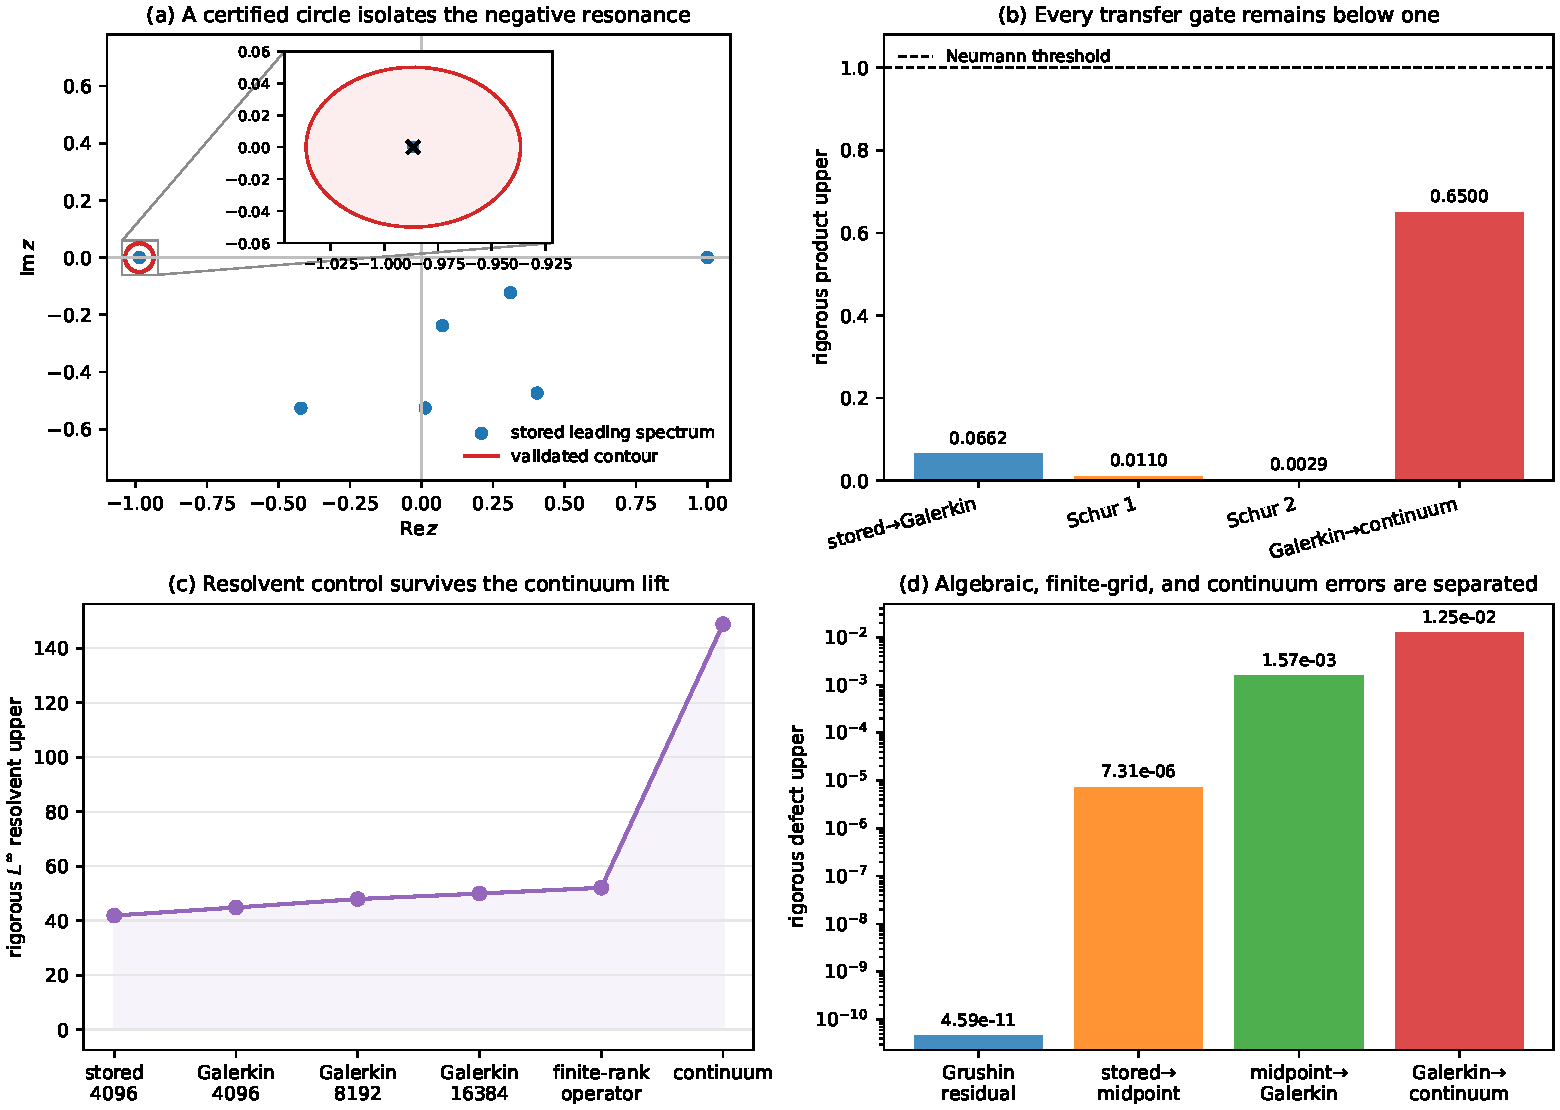
\includegraphics[width=\textwidth]{figures/validated_parity_continuum_contour.pdf}
\caption{The validated continuum lift.  (a) The blue leading-spectrum points
are a floating diagnostic from the preceding paper; the red circle is the
rigorous contour.  (b) Every rigorous Neumann or Schur transfer product is
below one.  (c) The $L^\infty$ resolvent upper remains controlled through
the stored, Galerkin, finite-rank, and continuum levels.  The final jump
includes the conservative continuum perturbation.  (d) Exact algebraic,
stored-to-midpoint, midpoint-to-Galerkin, and Galerkin-to-continuum defects
are recorded separately.}
\label{fig:summary}
\end{figure}

\section{Consequences and theorem boundary}
\label{sec:boundary}

The present result closes one precise gate and leaves several others
untouched.

\begin{enumerate}[leftmargin=2em]
 \item \textbf{Full-kernel parity simplicity is now proved.}
       At $\sigma=1/100$, the negative continuum resonance required by the
       weighted-Riesz theorem is real, algebraically simple, and isolated.
 \item \textbf{A continuum $L^\infty$ resolvent is explicit.}
       The same circle carries the uniform bound
       $148.84153451786617$.
 \item \textbf{The exact continuum-normalized midpoint family is controlled.}
       \Cref{cor:midpoint-family} supplies an explicit all-$n$ statement from
       $32768$ onward in the lifted $L^\infty$ norm.
 \item \textbf{Adaptive cutoff transfer is available in $L^\infty$.}
       Smooth discrete normalization converges at second order, while the
       adaptive support schedule of \citet{WangCutoff2026} has vanishing
       row-operator defect.  The resolvent perturbation theorem therefore
       transfers the isolated branch and its weighted Riesz term for all
       sufficiently fine adaptive grids in this norm.
 \item \textbf{No uniform Euclidean sparse-matrix theorem is claimed.}
       The $\ell^2$ condition required by the Euclidean cutoff proposition
       of \citet{WangRiesz2026} is a different statement.  Norm equivalence
       at a fixed dimension cannot be used uniformly as $n\to\infty$.
 \item \textbf{The noise width is fixed.}
       All derivative constants grow as $\sigma\downarrow0$.  No small-noise
       or double-limit theorem follows from the present constants.
\end{enumerate}

The center of the certified circle is a stored numerical datum, not a
closed-form expression for $\lambda_-$.  The theorem localizes the exact
continuum eigenvalue only to the real interval cut out by the circle.  It
does not connect that eigenvalue to a zeta zero, construct a self-adjoint
generator, prove a spectral counting law, or imply the Riemann hypothesis.

\section{Archive and reproducibility}
\label{sec:archive}

The repository archive separates three certificates:
\begin{enumerate}[leftmargin=2em]
 \item the exact-stored $4096$ Grushin contour certificate;
 \item the 224-bit Arb stored-to-exact-midpoint bridge; and
 \item the analytic Galerkin, Schur, and continuum composition certificate.
\end{enumerate}
Each cross-paper input is recorded by path and SHA-256 hash.  The final
archive additionally hashes all local sources, publication artifacts, and
the three result ledgers.

From the RH-41 directory, the complete replay is:
\begin{verbatim}
PYTHONDONTWRITEBYTECODE=1 /root/math/.venv/bin/python \
  -m pytest -q -p no:cacheprovider
PYTHONDONTWRITEBYTECODE=1 /root/math/.venv/bin/python \
  experiments/run_coarse_grushin_certificate.py
PYTHONDONTWRITEBYTECODE=1 /root/math/.venv/bin/python \
  experiments/build_midpoint_bridge_certificate.py
PYTHONDONTWRITEBYTECODE=1 /root/math/.venv/bin/python \
  experiments/build_continuum_certificate.py
MPLBACKEND=Agg PYTHONDONTWRITEBYTECODE=1 \
  /root/math/.venv/bin/python experiments/make_figures.py
latexmk -pdf -interaction=nonstopmode -halt-on-error main.tex
cp main.pdf validated-parity-continuum-contour.pdf
PYTHONDONTWRITEBYTECODE=1 /root/math/.venv/bin/python \
  experiments/build_archive.py
PYTHONDONTWRITEBYTECODE=1 /root/math/.venv/bin/python \
  experiments/verify_archive.py
\end{verbatim}

The Grushin replay is the expensive step because it validates the full
$4097$-dimensional bordered inverse in column chunks.  The Arb midpoint
bridge encloses all $4096$ rows.  The fast tests independently check the
closed-form bounds and every archived theorem gate.

\section{Conclusion}

The negative peripheral branch has now crossed the continuum-isolation
gate.  A one-center Grushin problem converts exact stored residuals into a
Rouch\'e count, Arb bridges the stored binary64 matrix to the exact analytic
midpoint kernel, exact-consistency Haar blocks propagate the contour through
two refinements, and a final $L^\infty$ perturbation closes the full
continuum operator.

The outcome is an exact fixed-noise theorem: one algebraically simple real
negative continuum resonance lies in the certified circle, and its contour
resolvent is explicitly bounded.  This supplies the missing premise for the
full-kernel weighted-Riesz parity bridge and yields an all-fine-grid
$L^\infty$ midpoint statement.  The route does not silently upgrade this
bound to a Euclidean sparse-matrix theorem and does not pass to zero noise.
Those are separate gates for later work.

\bibliographystyle{plainnat}
\small
\bibliography{references}

\end{document}
